%Induction and Heating are related to the gradient fields and the RF coils.
After briefly reviewing the image generation sequence, observe that it involves the primary components illustrated in Figure \ref{fig:scannerDesign}. These components are associated with various risks and safety concerns. Disregarding control systems and peripherals, the three main sources of hazard are the gradient coils, the \gls{rf} coils, and the main magnet, the latter presenting the most critical safety issues due to its powerful static magnetic field. 

%gradients safety concerns
\subsection{Hazards attributed to the encoding Gradient Fields}
\label{sec:gradients-induction-sound}
First, the quickly shifting magnetic gradients introduce hazard mechanisms beyond magnetic field strength. For example, when the gradient currents are repeatedly turned on and off, large forces called Lorentz forces, are applied to the coils in the strong magnetic field, leading to significant vibration. That, is the source of the loud "knocking" sounds during MR scans. Noise levels in modern \gls{mri} systems can easily exceed 130 dB, which is roughly a million times more intense in sound pressure than normal conversation or similar to an airplane taking off about 100 meters away, leading to temporary hearing loss as reported in early studies \cite{panych2018}. Consequently, hearing protection is now considered mandatory during MRI procedures.

Moreover, the rapid temporal variation of \gls{mri} gradient fields induces electric fields within conductive tissues via Faraday’s law. The effect scales with both the rate of change of the magnetic field and the spatial extent of the conductive path through tissue, so even though the absolute magnetic field perturbation from gradients (10–60 mT/m, or less than 1\% of $B_0$) is small, the rapid temporal ramping can induce voltages large enough to reach neural activation thresholds \cite{Davids:2017aa}. Typical clinical systems, limited by FDA guidelines to $\sim$ 40 T/s, remain below the threshold for cardiac excitation, but research systems capable of 300 mT/m gradients and higher slew rates approach that regime, posing theoretical cardiac stimulation risks \cite{bushberg2011, panych2018,Prince_MedicalImaging_2015}. Although these fields are much weaker than those associated with \gls{rf} transmission in terms of tissue heating the time-varying electric potentials can depolarize excitable membranes, producing \gls{pns} or, in extreme cases, involuntary muscle twitching \cite{panych2018,Grainger_MHRA_2014}.

%RF heating mechanism of action
\subsection{Heating as consequence of Radiofrequency pulses}
\label{sec:rf-heating}
Regarding the heating concern, the \gls{rf} field produced by an \gls{mri} scanner consists of both magnetic and electric components. Where, following Faraday's law, the time-varying magnetic field induces electrical currents within conducting loops or materials. Because there is a significant difference in electrical conductivity between the metallic implant and the surrounding human tissue, these currents experience Joule losses \cite{panych2018,aboyewa2021}. This energy is dissipated as heat directly into the adjacent tissue, causing a localized rise in temperature.

For straight metallic implants like epicardial leads, the antenna effect is a dominant mechanism for heating. The tangential component of the RF electric field that runs parallel to the lead causes free charges on the conductor's surface to migrate towards the tip of the lead. Then they accumulate creating a scattered electric field resulting in a much higher total electric field at the lead tips \cite{aboyewa2021,Langman2011}. Heating is further amplified if the physical length of the lead is comparable to the wavelength of the \gls{rf} pulse in the body. Here, the lead can act as a resonator, creating a standing wave of current along its length with maximum heating typically occuring when the lead length is approximately half the wavelength of the \gls{rf} frequency in tissue. For a 3 T MRI system, this resonant length is approximately 12–13 cm \cite{aboyewa2021}.

Finally, the extent of the heating action is determined by several variables, \gls{sar}, lead configuration, and lead structure. \gls{sar} is used to quantify the power deposited per unit mass in the tissue; higher SAR levels generally lead to higher temperature rises \cite{panych2018,aboyewa2021}. The shape, orientation, and termination significantly modify how the \gls{rf} field couples with the lead \cite{panych2018,aboyewa2021}.


\subsection{Risks associated with the Static Magnetic Field}
\label{sec:pull-fields}
In terms of the static magnetic field, the safety concerns are visible and much straight forward. The main magnet is the most distinguishing feature and is simultaneously the greatest source of risk associated with the device. This immense strength can cause everyday objects to behave in non-intuitive and dangerous ways, most notably turning ferromagnetic items into high-velocity projectiles \cite{panych2018}.

% Force and Torque 
A ferromagnetic object experiences a translational magnetic force that pulls it toward the scanner \cite{Schenck2000,panych2018} This force is not strongest at the center of the magnet. Rather, it is determined by the spatial gradient of the $B_0$ field. This aligns with theoretical insight of ASTM F2052-15 \cite{astmF2052}. Similarly, objects like those with asymmetric shapes, such as cylinders or needles, experience torque. Torque is the force that tries to twist an object so that its long axis aligns with the magnetic field lines and is dependent on this field with ASTM F2213-17 explaining some methodologies \cite{astm2213}. In the following section a derivation of the equations needed for the quantification and comparison of these forces is given.

In linear media, the magnetic flux density is directly proportional to the applied field strength. For magnetic dipoles $  \boldsymbol{m}  $ (or objects well-approximated as dipoles, such as cylindrical shapes), the mechanical interactions with the magnetic field, are governed by the following fundamental expressions from classical electromagnetism,

\begin{equation}
	\mathbf{F} = (\boldsymbol{m} \cdot \nabla)\mathbf{B}.
	\label{eq:force}
\end{equation}
\begin{equation}
	\boldsymbol{\tau} = \boldsymbol{m} \times \mathbf{B}.
	\label{eq:torque}
\end{equation}

\noindent where $\boldsymbol{m}$ is the magnetic dipole moment and $B$ is the magnetic field. 

These equations represent the general physics of dipole-field interactions and hold universally for induced or permanent dipoles in the low-susceptibility regime relevant to \gls{mri} safety testing. The torque expression (\ref{eq:torque}), in particular, is independent of any specific measurement protocol; however, its practical evaluation in the laboratory, such as the determination of $  \boldsymbol{m}  $ or the orientation relative to the field, depends on the experimental setup and will be detailed further in the context of our measurements.
For weakly paramagnetic materials, the induced magnetic moment magnitude can be estimated as

\begin{equation}
	m_0 = \frac{1}{\mu_0} \chi_m B_0 V.
	\label{eq:magnitudemoment}
\end{equation}

\noindent where where $  \chi  $ is the magnetic susceptibility, $  V  $ is the volume of the material, and $  \mu_0  $ is the permeability of free space. With these foundational expressions laid out, we can now develop the specific physical framework for the translational force relevant to our experimental setup.

\subsection{Translational Forces induced by the Static Field}
\label{sec:translationalForceBG}

In the \gls{mri} environment, the dominant safety concern for non-ferromagnetic objects arises not at isocenter, where the static field $ B_0  $ is uniform and $  \frac{dB_0}{dz} \approx 0  $, but in the fringe field region outside the bore, where strong spatial gradients exist.

Consider a simple pendulum with a metallic object at its end. This object is free to swing along the z-axis of an \gls{mri}. A static magnetic field along that same axis is then applied. The pendulum would be pulled towards the magnet with a force $F_m$ until it reaches equilibrium with its weight $mg$ and tension $T_s$. Figure \ref{fig:astm_diagram} shows a complete free body diagram.

\begin{figure}[htb!]
	\centering
	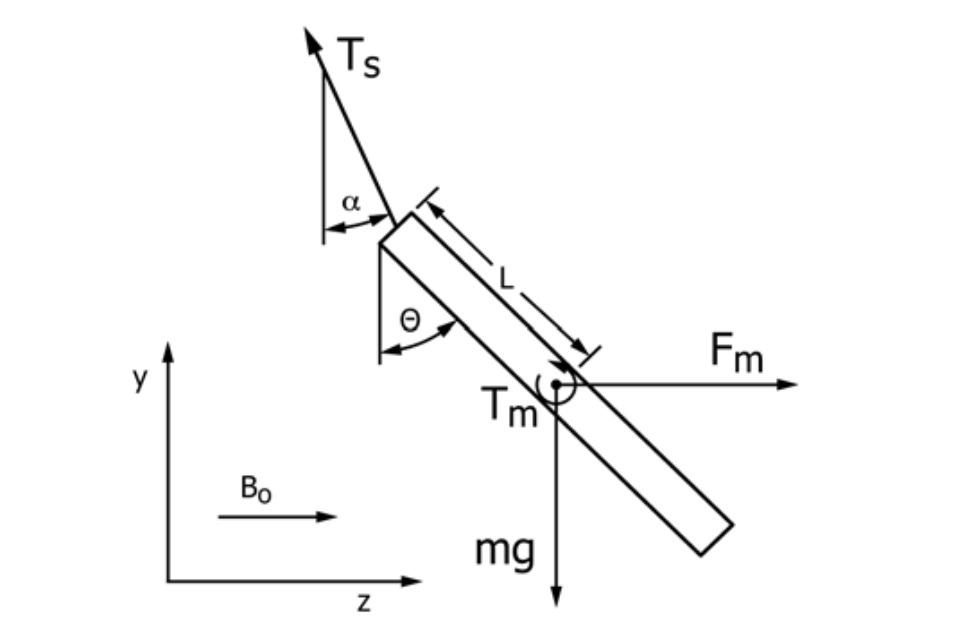
\includegraphics[width=0.4\textwidth]{Assets/astm_diagram.png}
	\caption[Free-body diagram of a metallic pendulum object in a static MRI magnetic field]{Free-body diagram of device in magnetic field (adapted from ASTM F2052-15 \cite{astmF2052}, Appendix X2).}
	\label{fig:astm_diagram}
\end{figure}

From Newton's laws at equilibrium point, the magnetic force can be found by measuring the angular deflection $\alpha$ such that 

\begin{equation}
	F_m = mg tan(\alpha). 
	\label{eq:Newton_translationalForce}
\end{equation}

Noting that this solution is independent of the point of attachment of the string and holds if the center of magnetic force does not coincide with the center of mass \cite{astmF2052}. On the other hand, by using Equations and \ref{eq:force} \ref{eq:magnitudemoment}, the magnetic force also is

\begin{equation}
	F_m =  \frac{\chi_m V}{\mu_0} B_0 \frac{dB_0}{dz}
	\label{eq:translationalForce}
\end{equation}

By comparing the magnetic force to the gravitational force ($F_g = m g$) the safety condition arises. If the device deflects less than $\alpha$ 45$^\circ$, then the magnetically induced deflection force is less than the force on the device due to its weight \cite{astmF2052}. This formulation explains why the measured deflection angle $\alpha$ (and thus $F_m$) depends not on $\chi$ or $B_0$ independently, but on their product. Practically, this insight justifies the lab methodology. Although magnets in our lab, a solenoid or neodymium magnets, generate small magnetic fields (only about 20 to 300 Gauss), we can use samples with proportionaly larger $\chi_m$ to replicate clinically relevant force-to-weight ratios ($F_m / F_g$). An estimation for the expected $\chi_m$ can be found on appendix \ref{app:scaling} and summarized in table \ref{tab:chi_scaling}.

%From equation (\ref{eq:forFit}), 
The measurable magnetic deflection depends on the ratio between the mechanical term and the magnetic force term. To reproduce the same deflection, 1 cm, at laboratory field strengths much smaller than those in MRI systems, the product must be preserved. Because $B_0 \nabla B_0 \propto B^2_0$ for a geometrically similar field, scaling the field down by a factor of  $10^2$ requires increasing the sample’s effective susceptibility by roughly $10^4$ to maintain the same mechanical response.

\begin{table}[htb]
	\centering
	\caption[Representative susceptibility scaling for laboratory solenoid fields.]{Values indicate the minimum magnetic susceptibility required to produce a measurable angular deflection (~1 cm over 1 m) under reduced field conditions (30–300 G and 3T), assuming a material density of ~7000 $kg/m^3$.}
	\label{tab:chi_scaling}
	\begin{tabular}{|c|c|c|c|}
		\hline
		$B_0$ (T) & $B\nabla B$ (T$^2$/m) & $\chi/\rho$ (m$^3$/kg) & $\chi_m$ (-) \\
		\hline
		$3.0 \times 10^{-3}$ & $1.707 \times 10^{-5}$ & $7.21 \times 10^{-3}$ & $5.05 \times 10^{\phantom{-}1}$ \\
		$3.0 \times 10^{-2}$ & $1.707 \times 10^{-3}$ & $7.21 \times 10^{-5}$ & $5.05 \times 10^{-1}$ \\
		$3.0 \times 10^{\phantom{-}0}$  & $1.707 \times 10^{\phantom{-}1}$  & $7.21 \times 10^{-9}$ & $5.05 \times 10^{-5}$ \\
		\hline
	\end{tabular}
\end{table}

For typical solenoids producing 30–300 G, the factor of $\chi_m/\rho$ spans from approximately one hundred-thousandth to one-thousandth of that found in ferromagnetic materials. Consequently, to appropriately mimic translational forces under these laboratory conditions, a realistic value of $\chi_m$ for a substitute should lie between one and ten. For example, a nonmagnetic stainless steel wire ($\chi_m \approx 10^{-4}$) might show a magnetic force of 30\% of the object's weight, whereas ferromagnetic metals like nickel can exceed two million percent. That is more than enough to become dangerous projectiles unless restrained \cite{aboyewa2021,Woods2021_MRIdisplacement,panych2018}.



In the other hand, the effect of the static field on torque are expected to be less significant that the pull as it only dependent on the field strength and not its gradient. As the curl is decomposed into the torque magnitude we observe that only components parallel to the field have an effect on the it, with that in mind lets address the problem.

\subsection{Torque induced by the Static Field}
\label{sec:torqueBG}

Consider a metallic rigid cylinder shaped subject (a wire or rod) free to rotate, in a low friction surface, and align itself to a static magnetic field ($B_0$). The cylinder experiences a torque and has magnetic dipole moment according to eq. (\ref{eq:torque}). For a thin, linear paramagnetic material, the induced magnetic moment depends on its orientation relative to the static magnetic field. It can be expressed as

\begin{equation}
	\mathbf{m} = m_0 \cos (\theta),
	\label{eq:mprojection}
\end{equation}

\noindent where $m_0$ is the maximum induced dipole moment, which occurs when the material’s axis is aligned parallel to the $B_0$ field ($\theta$ = 0$^\circ$). When the material is oriented perpendicular to $B_0$ ($\theta$ = 90$^\circ$), the effective component of the dipole moment along the field direction vanishes. This follows from the projection of the dipole moment vector onto the magnetic field axis.

\begin{figure}[htb!]
	\centering
	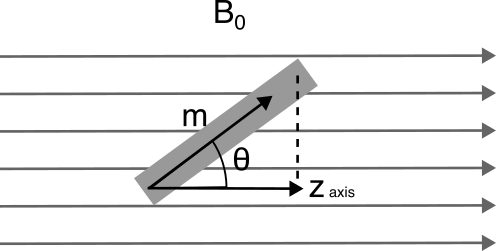
\includegraphics[width=0.65\textwidth]{Assets/dipole.png}
	\caption{Vector diagram of a magnetic dipole $\mathbf{m}$ in a uniform magnetic field $\mathbf{B}$ directed along the $z$-axis.}
	\label{fig:m0mcost}
\end{figure}

In Figure \ref{fig:m0mcost}, the dipole of length $a$, experiences a torque magnitude $|\boldsymbol{\tau}| = |\mathbf{m} \times \mathbf{B}| = m B_0 \sin\theta$. From the geometric projection of the dipole moment onto the magnetic field direction (eq. \ref{eq:mprojection}), and the torque experienced by the dipole we can write
\begin{equation*}
	|\boldsymbol{\tau}| = m_0 B_0 \sin(\theta) \cos(\theta) = m_0 B_0 \frac{\sin (2\theta)}{2}.
\end{equation*}

Using equation \ref{eq:magnitudemoment} for the dipole moment, we then write 

\begin{subequations}
	\begin{equation}
		\tau(\theta) = \tau_{max} \sin(2\theta), \text{or}
		\label{eq:torque_thetadependece}
	\end{equation}
	\begin{equation}
		\tau_{max} = \frac{\chi_m B_0^2 V}{2 \mu_0}.
		\label{eq:maxtorque}
	\end{equation}
	\label{eq:magnetic_torque}
\end{subequations}

Once the torque is found, a direct comparison to the body's weight can be made. According to ASTM F2213 \cite{astm2213, stoianovici2024}, the criterion ($c_\tau$) for evaluating magnetically induced torque on medical devices in a magnetic resonance environment is

\begin{equation}
	c_\tau = \frac{\tau_{max}}{mgL},
	\label{eq:gravTorque}
\end{equation} 

\noindent where $\tau_{max}$ is the maximum torque measured or obtained by equation \ref{eq:maxtorque}, meaning that the maximum magnetically induced torque is comparable than the product of the device's longest dimension ($L$) and its weight ($mg$). Under the ASTM gravity-based acceptability criterion, a device is considered acceptable when $c_\tau < 1$.